\documentclass[aspectratio=169,10pt]{beamer}
\usepackage[utf8]{inputenc}
\usepackage[T1]{fontenc}
\usepackage{lmodern}
\hyphenpenalty=10000
\exhyphenpenalty=10000
\usepackage{booktabs,graphicx,amsmath}
\definecolor{navy}{HTML}{142B43}
\definecolor{teal}{HTML}{007F83}
\definecolor{orange}{HTML}{B55A21}
\definecolor{muted}{HTML}{526273}
\setbeamercolor{normal text}{fg=navy,bg=white}
\setbeamercolor{frametitle}{fg=navy}
\setbeamercolor{structure}{fg=teal}
\setbeamercolor{alerted text}{fg=orange}
\setbeamercolor{block title}{fg=teal,bg=white}
\setbeamercolor{block body}{fg=navy,bg=white}
\setbeamertemplate{navigation symbols}{}
\setbeamertemplate{frametitle}{\vspace{0.15cm}\insertframetitle\par\vspace{0.03cm}{\color{teal}\rule{\textwidth}{0.6pt}}}
\setbeamersize{text margin left=0.6cm,text margin right=0.6cm}
\setbeamerfont{frametitle}{size=\Large,series=\bfseries}
\setbeamerfont{footline}{size=\tiny}
\setbeamertemplate{footline}{\hspace{0.6cm}\color{muted}EAD6034 | Renan de Luca Avila | 21/09/2026\hfill\insertframenumber/7\hspace{0.6cm}\vspace{0.15cm}}
\hypersetup{colorlinks=true,urlcolor=teal,linkcolor=teal,pdftitle={EAD6034 | Entrega cumulativa de 21/09/2026},pdfauthor={Renan de Luca Avila}}
\newcommand{\source}[2]{\par\vfill{\raggedright\tiny\color{muted}#1\quad\href{#2}{Código reproduzível no GitHub}\par}}
\newcommand{\tagline}[1]{{\small\color{teal}#1}\par\medskip}
\begin{document}
\begin{frame}[t]{Dois anos, seis escalas, uma regra temporal}
\tagline{Previsibilidade linear do WIN: 31/08 + 14/09 + 21/09}
\begin{columns}[T]\begin{column}{0.48\textwidth}
\textbf{Pergunta:} agregar minutos em horas melhora a previsão dos retornos?\medskip\par
Treino: \textbf{2024}, 246 pregões.\par Teste: \textbf{2025}, 221 pregões.\medskip\par
Janela comum: 09:05--18:05.\par Retornos logarítmicos em \%.\medskip\par
\alert{Não criamos retorno overnight.}\par Os lags e estados \textbf{continuam} entre pregões, em tempo de negociação.
\par\medskip\scriptsize\href{https://alphalab.btgpactual.com/datasets/publication:7a74b3ae-90e0-4393-b1e0-01e61c0bedba}{Fonte: BTG Alpha Lab | BTG-ATS-A26}\par Candles de negócios B3. Contrato de maior volume do próprio dia: seleção retrospectiva.\end{column}\begin{column}{0.47\textwidth}\centering\scriptsize
\begin{tabular}{lrr}
\toprule
Escala & $n$ treino & $n$ teste \\ \midrule
1 min & 132.840 & 119.340 \\
5 min & 26.568 & 23.868 \\
15 min & 8.856 & 7.956 \\
30 min & 4.428 & 3.978 \\
60 min & 2.214 & 1.989 \\
Diário OC & 246 & 221 \\
\bottomrule
\end{tabular}\par
\smallskip\scriptsize 02/01--30/12/2024; 02/01--28/11/2025.\par Diário: abertura--fechamento da janela.\par 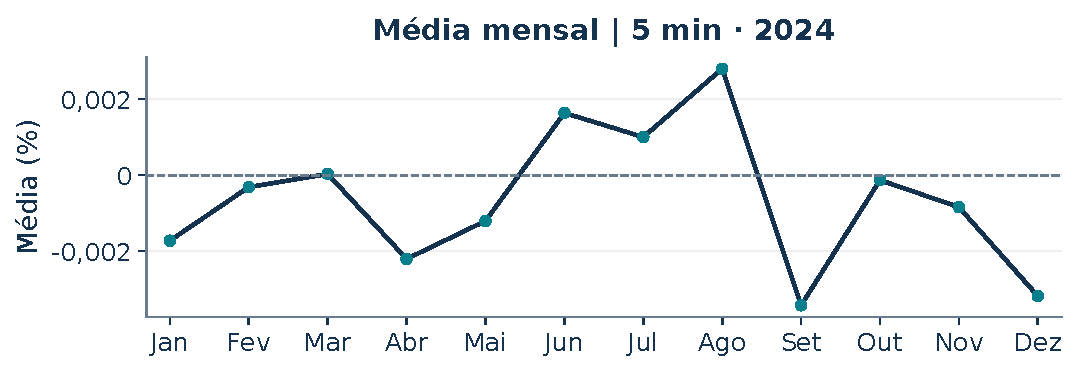
\includegraphics[width=\textwidth,height=2.05cm,keepaspectratio]{figures/08_monthly_mean_5min.pdf}\par \tiny Média dos retornos de 5 min, não retorno mensal acumulado.\end{column}\end{columns}
\source{Dados e protocolo | 31/08 revisado}{https://github.com/avilarenan/EAD6034/blob/6e24660054ee39c6037fc1e68aed22d4b78ea6ed/src/ead6034/trading_time_data.py}
\end{frame}

\begin{frame}[t]{Da descrição às hipóteses de dependência}
\tagline{31/08: identificação refeita com a sequência anual de 2024}
\centering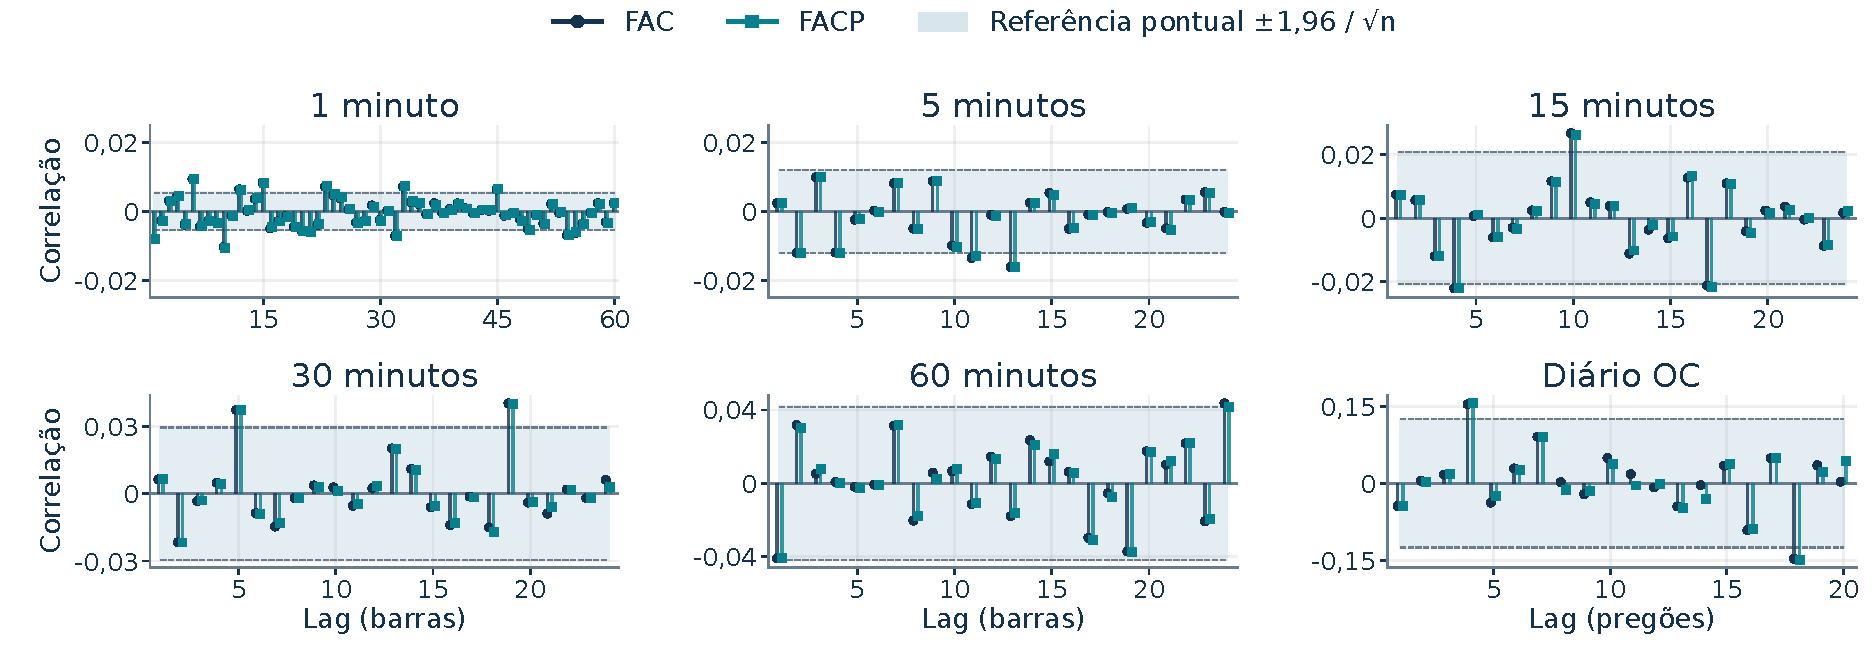
\includegraphics[width=0.98\textwidth,height=5.0cm,keepaspectratio]{figures/01b_return_acf_pacf_slide.pdf}\par\smallskip 
\scriptsize Um lag = uma barra da própria escala, inclusive entre pregões. Bandas pontuais não corrigem múltiplas comparações.\par Dispersão e dependência na média são propriedades distintas.\par Desvios-padrão (\%; 1/5/15/30/60 min/diário): 0,032; 0,071; 0,122; 0,171; 0,245; 0,785.
\source{Aulas 2--4 | FAC/FACP convencionais}{https://github.com/avilarenan/EAD6034/blob/6e24660054ee39c6037fc1e68aed22d4b78ea6ed/src/ead6034/annual_models.py}
\end{frame}

\begin{frame}[t]{Estacionariedade: uma série anual por escala}
\tagline{14/09 revisado: inferência com toda a amostra de 2024}
\centering\small\begin{tabular}{lrrrrr}
\toprule
Escala & $n$ & $p$ ADF & $p$ PP & $p$ KPSS & Lags/bw* \\ \midrule
1 min & 132.840 & $<0{,}001$ & $<0{,}001$ & 0,290 & 0/73/15 \\
5 min & 26.568 & $<0{,}001$ & $<0{,}001$ & 0,286 & 0/49/7 \\
15 min & 8.856 & $<0{,}001$ & $<0{,}001$ & 0,273 & 0/37/11 \\
30 min & 4.428 & $<0{,}001$ & $<0{,}001$ & 0,274 & 0/31/6 \\
60 min & 2.214 & $<0{,}001$ & $<0{,}001$ & 0,270 & 0/27/2 \\
Diário OC & 246 & $<0{,}001$ & $<0{,}001$ & 0,334 & 0/16/0 \\
\bottomrule
\end{tabular}\par
\raggedright\medskip\small ADF e PP: $H_0$ = raiz unitária. KPSS: $H_0$ = estacionariedade em nível.\par\medskip\textbf{A correção central:} 60 min passa de 9 por pregão para 2.214 observações anuais.\par\scriptsize *Ordem ADF/PP/KPSS. Constante: especificação principal acima.\par \alert{Sensibilidade: KPSS com tendência rejeita em 6 das seis escalas.}\par Não rejeitar KPSS não prova estabilidade de toda a distribuição; a variância pode variar.
\source{Aula 5 | Estatísticas e valores críticos nas tabelas completas}{https://github.com/avilarenan/EAD6034/blob/6e24660054ee39c6037fc1e68aed22d4b78ea6ed/src/ead6034/annual_models.py}
\end{frame}

\begin{frame}[t]{BIC seleciona; os resíduos ainda precisam passar}
\tagline{14/09 revisado: grade $p,q=0,\ldots,5$, média e variância contadas no BIC}
\centering\small\begin{tabular}{lrrrr}
\toprule
Escala & ARMA BIC & Alternativos & $p$ Ljung--Box & $p$ ARCH--LM \\ \midrule
1 min & (2,2) & AR(1) / MA(1) & $<0{,}001$ & $<0{,}001$ \\
5 min & (0,0) & AR(1) / MA(1) & 0,078 & $<0{,}001$ \\
15 min & (0,0) & AR(1) / MA(1) & 0,410 & $<0{,}001$ \\
30 min & (0,0) & AR(1) / MA(1) & 0,498 & $<0{,}001$ \\
60 min & (0,0) & AR(1) / MA(1) & 0,366 & $<0{,}001$ \\
Diário OC & (0,0) & AR(1) / MA(1) & 0,399 & $<0{,}001$ \\
\bottomrule
\end{tabular}\par
\raggedright\medskip\small \textbf{Seleção não é validação.} Ljung–Box rejeita em 1 min.\par\smallskip\scriptsize Minuto: vantagem de apenas $\Delta BIC=1,24$ sobre (0,0); candidato sem validação residual.\par 5 min: não rejeita em 24 lags, mas rejeita em 10, 12 e 20. AR e MA são as alternativas lineares.\par\smallskip \scriptsize Diagnósticos assintóticos aproximados sob heteroscedasticidade. Q usa $h-p-q-1$ (Aula 4); $h=60$ em 1 min, 24 nas demais intradiárias, 20 no diário.
\source{Aulas 3--4 | Box--Jenkins e alternativas lineares}{https://github.com/avilarenan/EAD6034/blob/6e24660054ee39c6037fc1e68aed22d4b78ea6ed/src/ead6034/annual_models.py}
\end{frame}

\begin{frame}[t]{Prever a variância não é prever a direção}
\tagline{Aula 6: constante, ARCH(1) e GARCH(1,1), escolhidos apenas em 2024}
\centering\small\begin{tabular}{lrrrr}
\toprule
Escala & Variância BIC & $\alpha+\beta$ & $p$ Q($z^2$)* & MSE/const.* \\ \midrule
1 min & GARCH(1,1) & 0,987 & $<0{,}001$ & 0,955 \\
5 min & GARCH(1,1) & 0,899 & 1,000 & 0,970 \\
15 min & GARCH(1,1) & 0,696 & 1,000 & 0,908 \\
30 min & GARCH(1,1) & 0,450 & 0,300 & 0,973 \\
60 min & ARCH(1) & 0,144 & 0,013 & 0,984 \\
Diário OC & Constante & 0,000 & 0,003 & 1,000 \\
\bottomrule
\end{tabular}\par
\raggedright\medskip\small Estimação \textbf{sequencial}; previsão pontual do retorno \textbf{não muda}.\par BIC não atesta adequação: rejeições em Q($z^2$) sinalizam dependência restante.\par\medskip\scriptsize *Q dos resíduos padronizados ao quadrado no maior lag exibido. MSE em 2025 contra inovação ao quadrado: proxy ruidosa, não variância observada.\par Captura parcial: minuto, hora e diário ainda rejeitam em Q($z^2$). BIC é condicional à média fixa.
\source{Aula 6 | Estabilidade, persistência e diagnóstico}{https://github.com/avilarenan/EAD6034/blob/6e24660054ee39c6037fc1e68aed22d4b78ea6ed/src/ead6034/conditional_volatility.py}
\end{frame}

\begin{frame}[t]{A comparação justa usa o mesmo alvo futuro}
\tagline{21/09: parâmetros fixos de 2024, somente informação passada em cada origem}
\centering\small\begin{tabular}{lrrrrr}
\toprule
Escala & ARMA & AR & MA & 50/50 & $p$ DM \\ \midrule
1 min & 1,0019 & 1,0021 & 1,0021 & 1,0021 & 0,114 \\
5 min & 1,0020 & 1,0020 & 1,0020 & 1,0020 & 0,973 \\
15 min & 1,0020 & 1,0022 & 1,0022 & 1,0022 & 0,406 \\
30 min & 1,0020 & 1,0022 & 1,0022 & 1,0022 & 0,437 \\
60 min & 1,0020 & 1,0029 & 1,0028 & 1,0029 & 0,470 \\
Diário OC* & 1,0170 & 1,0193 & 1,0195 & 1,0194 & 0,554 \\
\bottomrule
\end{tabular}\par
\raggedright\medskip\small \textbf{MSE do modelo / MSE do retorno zero: menor que 1 é melhor.}\par Intradiário: 1.989 alvos idênticos de 60 minutos, sem sobreposição.\par\scriptsize *Diário prevê sua janela open-to-close: alvo diferente, não entra no ranking intradiário.\par DM compara apenas AR versus MA, não ARMA versus zero. Referência aproximada; p-valores sem ajuste de multiplicidade. Perdas absolutas e horizonte nativo estão no relatório.
\source{Aula 4 | MSE, MAE, combinação e Diebold--Mariano}{https://github.com/avilarenan/EAD6034/blob/6e24660054ee39c6037fc1e68aed22d4b78ea6ed/src/ead6034/forecast_evaluation.py}
\end{frame}

\begin{frame}[t]{Conclusão: alcance dos resultados e da metodologia}
\tagline{A hipótese de maior previsibilidade horária não recebeu suporte neste desenho}
\small\textbf{Evidência:} ARMA no alvo comum tem 0,194\% (1 min) e 0,203\% (60 min) mais MSE que zero. Diferença descritiva; DM compara AR com MA.\par\medskip\begin{columns}[T]\begin{column}{0.50\textwidth}\small\textbf{ARMA de 60 min em 2025}\par\smallskip\begin{tabular}{lrr}
\toprule
Recorte & $n$ & MSE/zero \\ \midrule
Início & 221 & 1,0009 \\
Meio & 1547 & 1,0022 \\
Fim & 221 & 1,0036 \\
Gap alto & 873 & 1,0019 \\
Gap baixo & 1026 & 1,0031 \\
\bottomrule
\end{tabular}\par
\scriptsize Início: 09:05--10:05; meio: até 17:05; fim: até 18:05. Todas as escalas no relatório.\par Grupos não são aditivos; gaps indisponíveis excluídos desse recorte.\end{column}\begin{column}{0.46\textwidth}\small\textbf{Força:} mesmos alvos e parâmetros fixados antes do teste.\par\smallskip \textbf{Limites:} contrato escolhido por volume diário e dias completos são seleções retrospectivas.\par\smallskip \alert{Leilões: mecanismos plausíveis, sem identificação causal.}\par\smallskip \scriptsize Overnight fora do alvo, mas lags continuam. Sem flags de fase; horários históricos incompletos.\par\smallskip Dependência da variância não garante direção previsível. Resultado restrito a este ativo, janela e modelos; não prova eficiência de mercado ou lucro após custos.\end{column}\end{columns}\medskip\scriptsize\href{https://github.com/avilarenan/EAD6034/blob/main/results/entrega_21_09/RELATORIO_21_09.md}{Relatório, análises por faixa/gap e resultados completos}

\source{Síntese cumulativa | Evidência, adequação e utilidade econômica são distintas}{https://github.com/avilarenan/EAD6034/blob/6e24660054ee39c6037fc1e68aed22d4b78ea6ed/src/ead6034/forecast_pipeline.py}
\end{frame}

\end{document}
